\documentclass[../main.tex]{subfiles}


\begin{document}
\section{The warmest and coldest days of the year}
	The task is to find the warmest and coldest day for a number of different years. The data is analysed by first using a for loop which will go through all values in the dataset. For every data point the temperature is checked and if it is higher than the previously highest temperature for the year, the day, temperature and month of that day is recorded. This is also done for the coldest days and an example of the code can be seen below.
	\vspace{2mm}
	\begin{lstlisting}[frame=single] 
for (k = 0; (unsigned)k < (year.size()-1); k++) { 
	if (temperature.at(k) > hottest){ 
		hottest = temperature.at(k);
		hottestDay = day.at(k);
		hottestMonth = month.at(k);
	}
}
	\end{lstlisting}
	\vspace{2mm}
	At the end of each year the highest and coldest days are saved inside vectors which will be used later. These vectors are used to fill three separate histograms. One for the warmest days, one for the coldest days in the beginning of the year and one for the coldest days at the end of the year. The coldest days are separated to make the guassian fit work.\\
	
	With the values in histograms the histograms are plotted in the same canvas and guassian fits are applied. By using guassian fits we can obtain a mean for the warmest and coldest days and also the uncertainties of these values. By using the Lund dataset, shown in figure \ref{hotColdPlot}, we can see that the mean of the warmest day is: $196\pm3$ and for the coldest day: $24\pm8$. These results shows that the warmest day is most likely to occur in the middle of June and the coldest day is most likely to occur in the end of January.
	
	\begin{figure}[h]
		\centering
		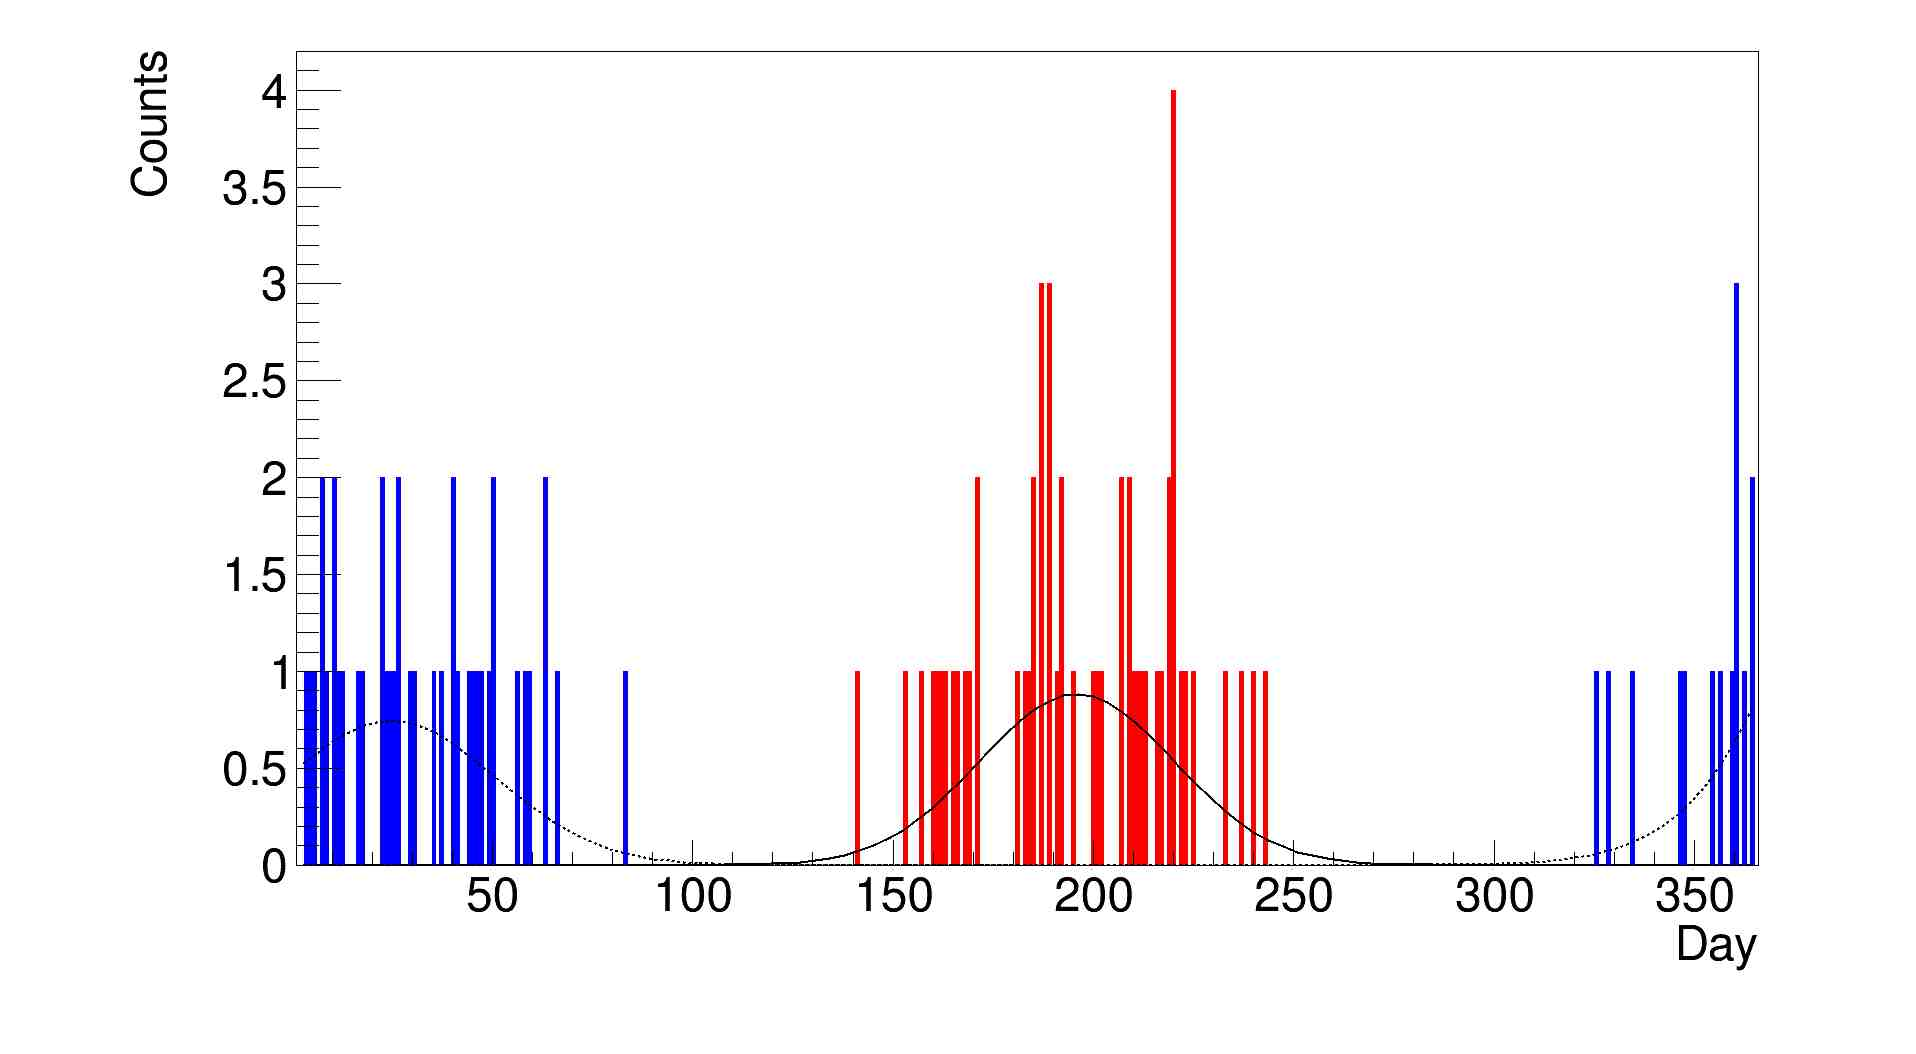
\includegraphics[width=1.2\textwidth] {hotColdDays.jpg}
		\caption{Plot of the warmest and coldest days for each year. 		Also a guassian fit for both.}
		\label{hotColdPlot}
	\end{figure}
\end{document}